\documentclass[12pt,a4paper]{article}
\usepackage[utf8]{inputenc}
\usepackage[english,russian]{babel}
\usepackage[T1, T2A]{fontenc}
\usepackage{graphicx}
\usepackage{epstopdf}
\usepackage{caption, subcaption}
\usepackage{threeparttable}
\usepackage[margin=14pt,font=small,labelsep=endash]{caption}
\captionsetup[table]{name = Таблица, labelsep = endash, justification=raggedright, singlelinecheck=false}
\captionsetup[figure]{labelformat=simple, labelsep = endash, name = Рисунок}
\usepackage{float}
\usepackage{geometry} %способ ручной установки полей
\geometry{top=2cm} %поле сверху
\geometry{bottom=2cm} %поле снизу
\geometry{left=2cm} %поле справа
\geometry{right=2cm} %поле слева
\usepackage{amsmath}
\newcommand\tline[2]{$\underset{\text{#1}}{\text{\underline{\hspace{#2}}}}$}
\newcommand\nameLine[3]{$\underset{\text{#1}}{\text{\underline{\text{#2}\hspace{#3}}}}$}
\renewcommand{\arraystretch}{2}

\begin{document}
	\begin{titlepage}
		\centering
		{\fontsize{12pt}{5cm}\selectfont \bfseries Министерство образования и науки Российской Федерации} \\ \vspace{0.5cm}
		{\fontsize{7pt}{5cm}\selectfont ФЕДЕРАЛЬНОЕ ГОСУДАРСТВЕННОЕ АВТОНОМНОЕ ОБРАЗОВАТЕЛЬНОЕ УЧРЕЖДЕНИЕ ВЫСШЕГО ПРОФЕССИОНАЛЬНОГО ОБРАЗОВАНИЯ} \\ 
		\vspace{1cm}
		{\fontsize{12pt}{5cm}\selectfont \bfseries САНКТ-ПЕТЕРБУРГСКИЙ УНИВЕРСИТЕТ ИНФОРМАЦИОННЫХ ТЕХНОЛОГИЙ, МЕХАНИКИ И ОПТИКИ} \\ \vspace{1.5cm}

		{\fontsize{14pt}{5cm}\selectfont Кафедра \hspace{1cm} \underline{Систем Управления и Информатики}  \hspace{1cm} Группа \underline{Р3340}} \\ 
		\vspace{2cm}

		{\fontsize{20pt}{5cm}\selectfont \bfseries Лабораторная работа №7} \\
		{\fontsize{20pt}{5cm}\selectfont \bfseries Анализ точности систем управления} \\
		{\fontsize{14pt}{5cm}\selectfont Вариант - 9} \\
		\vspace{1.5cm}

		\flushleft

		{Выполнила \hspace{1,7cm} \nameLine{(фамилия, и.о.)}{Сорокина Т. В.}{6.3cm} (подпись)} \\
		\vspace{2cm}

		{Проверил \hspace{2cm} \tline{(фамилия, и.о.)}{9cm} (подпись)} \\
		\vspace{5cm}

		"\underline{\hspace{0.7cm}}"\hspace{0.2cm}\underline{\hspace{2cm}}\hspace{0.2cm}20\underline{\hspace{0.7cm}}г. \hspace{2cm} Санкт-Петербург, \hspace{2cm} 20\underline{\hspace{0.7cm}}г. \\ \vspace{1cm}

		Работа выполнена с оценкой \hspace{1cm} \underline{\hspace{8cm}} \\ 
		\vspace{1cm}
		Дата защиты "\underline{\hspace{0.7cm}}"\hspace{0.2cm}\underline{\hspace{2cm}}\hspace{0.2cm}20\underline{\hspace{0.7cm}}г.

	\end{titlepage}

%opening
%\title{}
%\author{}

 \par
\paragraph{Цель работы:} исследование точностных свойств систем управления.
\par
В задании требуется провести исследование системы с астатизмом нулевого порядка и с астатизмом первого порядка.
Исследовать стационарный режим работы: g(t)=A, и режим движения с постоянной скоростью: g(t)=Vt и режим движения с постоянным ускорением $g(t)=at^2/2$.
\par 
Получить переходные процессы для различных значений коэффициента k. 
Определить предельное значение установившейся ошибки $\varepsilon$.\\
\textbf{Исходные данные}
\par В таблице 1 представлены  параметры системы: передаточная функция объекта управления, характеристики задающих и возмущающих воздействий. 

\begin{table} [h!]
\centering
\begin{threeparttable}
\caption{Исходные данные}
\begin{tabular}{ |c|c|c|c|c|c|c|c| }
 \hline
  W(s) & g=A & g=Vt &  $g=at^2/2$ & Структура системы & $f_{1}$ & $f_{2}$ & Сигнал задания \\ 
 \hline
  $ 2/(0.5s^2+s+2) $ & 2 & 2t  & $ 0.5t^2 $ & в) & 2 & 0.5 & $2+0.1t^2$ \\ 
 \hline
\end{tabular}
\end{threeparttable}
\end{table}


\newpage
\begin{center}
\section{Исследование системы с астатизмом нулевого порядка}
\end{center}
\par На рисунке 1 представлена структурная схема моделируемой системы.

\begin{figure}[h!]
\centering
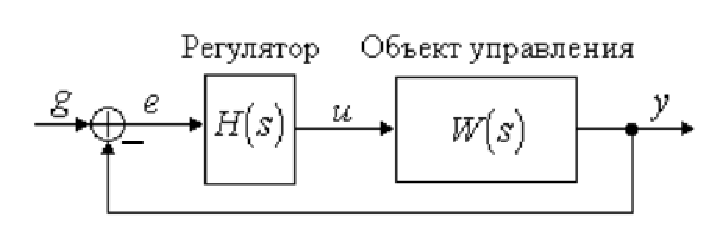
\includegraphics[width=0.5\textwidth]{1/22.eps} 
\caption{Структурная схема моделируемой  системы нулевого порядка}
\end{figure}

\subsection{Исcледование стационарного режима работы: $g(t)=A$}

Значение коэффициентов k: 1, 5, 10.
На рисунке 2 представлена структурная схема моделируемой системы нулевого порядка.
\begin{figure}[h!]
\centering
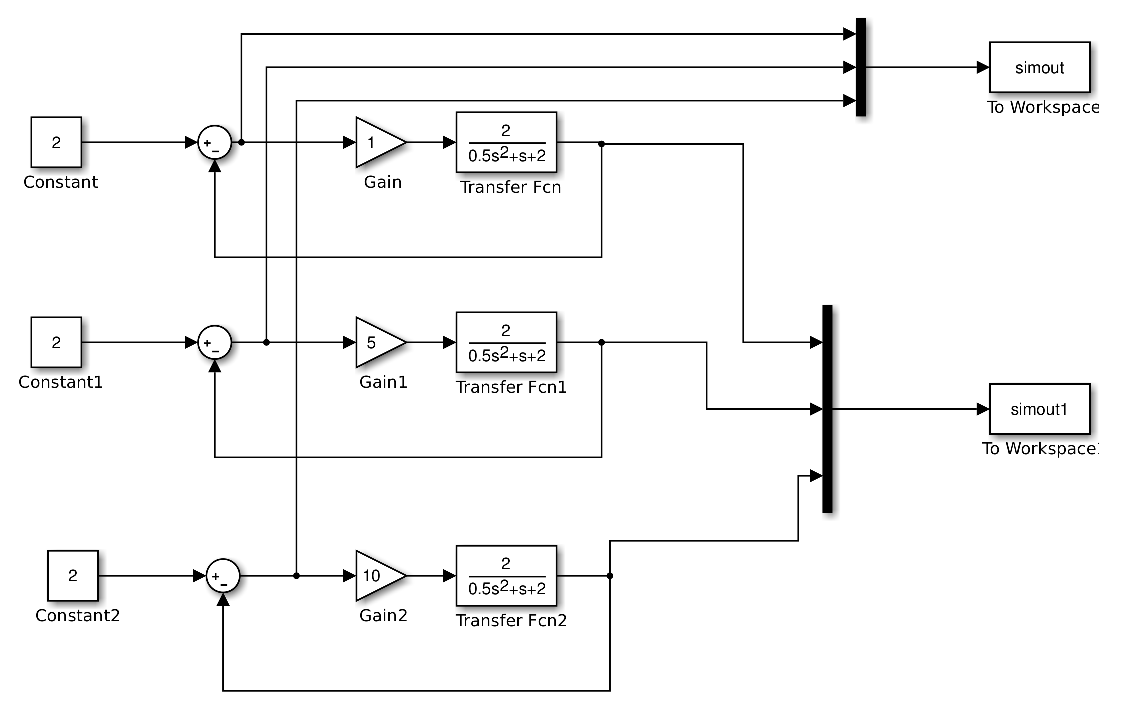
\includegraphics[width=\textwidth]{1/1_1.eps} 
\caption{Структурная схема моделируемой  системы нулевого порядка}
\end{figure}

Получили переходные процессы для трех различных значений коэффициентов k (k=1; k=5; k=10).
На рисунке 3 представлены графики переходного процесса для k=1; k=5; k=10.
\begin{figure}[H]
\centering
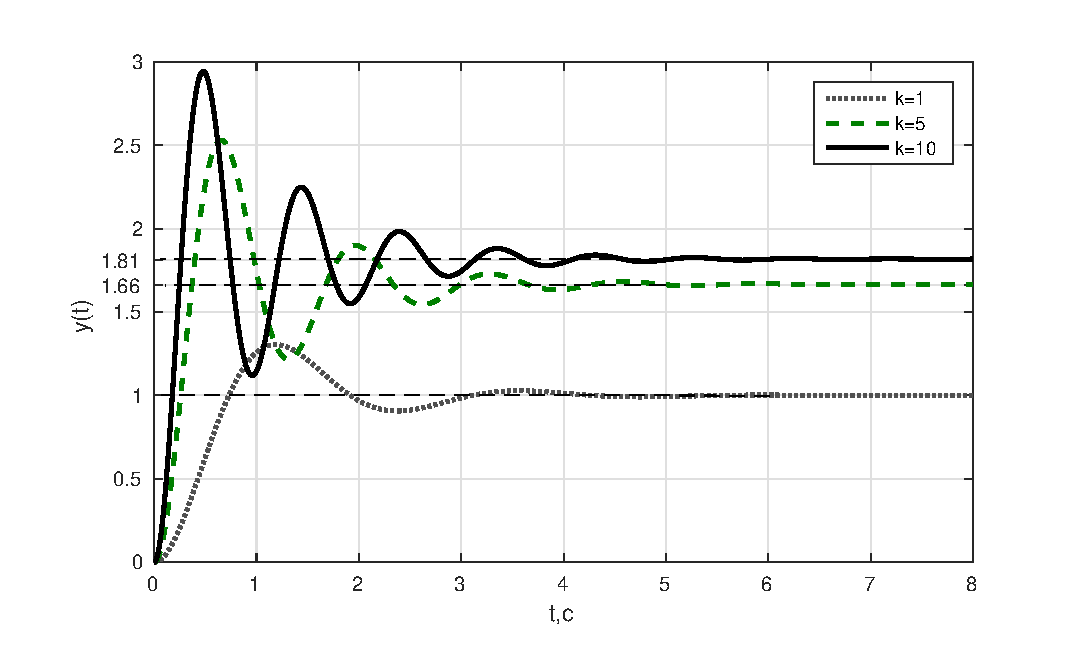
\includegraphics[width=\textwidth]{1/1_1y(t).eps}
\caption{Графики переходного процесса для k=1; k=5; k=10}
\end{figure}

Было получено предельное значение установившейся ошибки е. На рисунке 4 приведены графики, изображающие предельное значение установившейся ошибки. 
\begin{figure}[H]
\centering
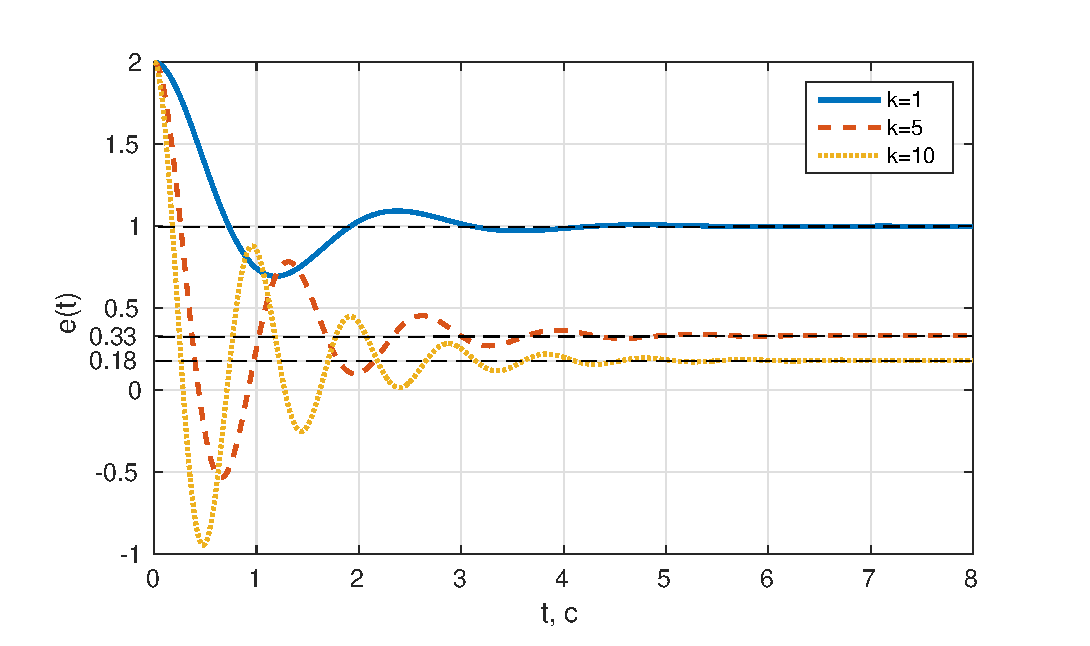
\includegraphics[width=\textwidth]{1/1_1e.eps}
\caption{Графики, изображающие предельное значение установившейся ошибки}
\end{figure}

\newpage
С помощью расчета проверим получившееся на графике значения установившейся ошибки:
\begin{equation}
e=\frac{A}{(1+k)}
\end{equation}
Подставим полученные значения:
\\при k=1: e=2/(1+1)=1
\\при k=5: e=2/6=1/3=0.33
\\при k=10: e=2/11=0.18.

Рассчитанные значения совпадают с получившимися значениями на графике.

\subsection{Исследование режима движения с постоянной скоростью: \\$g(t)=Vt$}

На рисунке 5 представлена структурная схема моделируемой системы.
\begin{figure}[H]
\centering
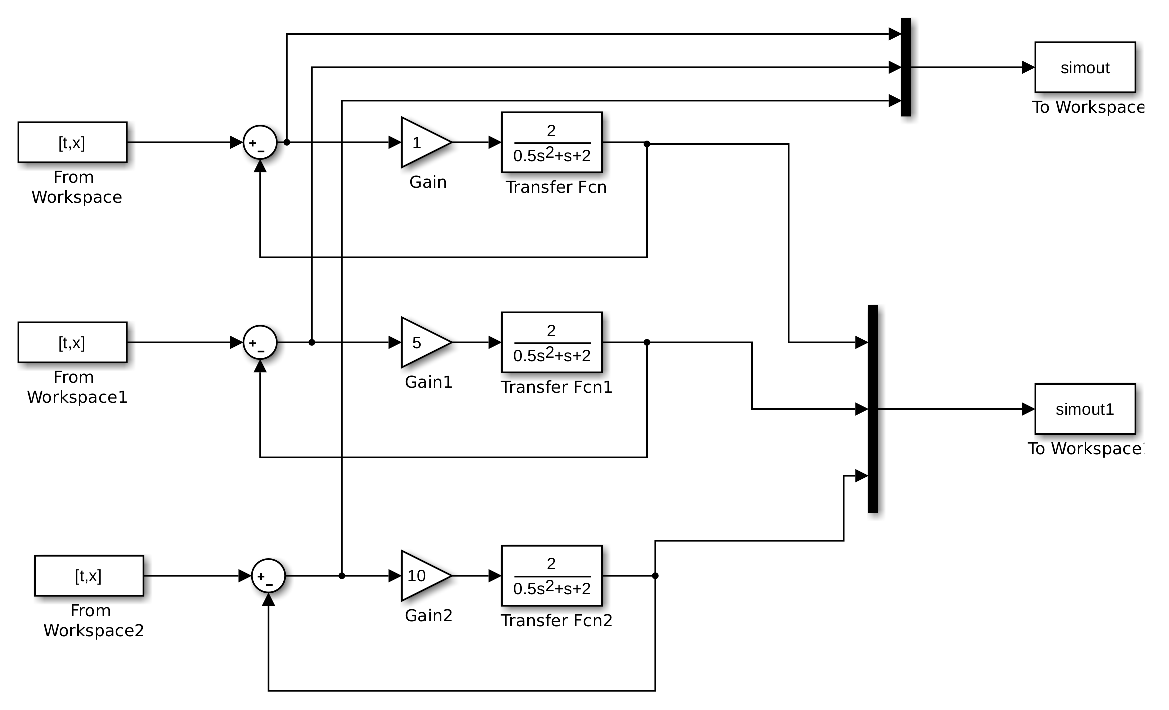
\includegraphics[width=\textwidth]{1/1_2.eps}
\caption{Структурная схема моделируемой  системы}
\end{figure}

Получили переходные процессы для трех различных значений коэффициентов k (k=1; k=5; k=10).
\begin{figure}[H]
\centering
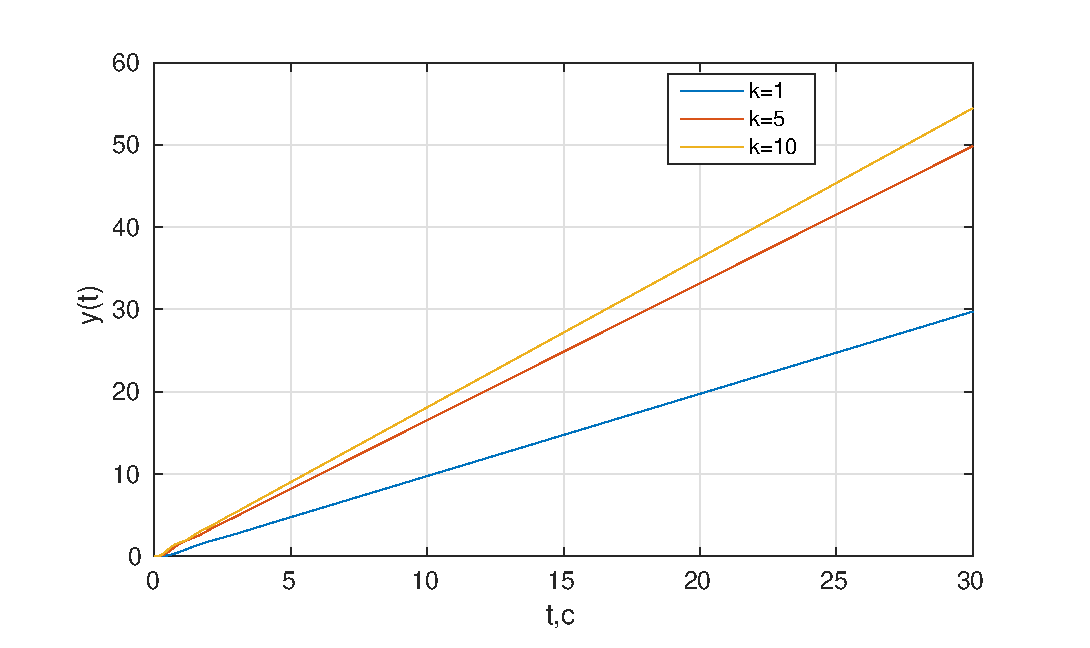
\includegraphics[width=\textwidth]{1/1_2y(t).eps}
\caption{Графики переходного процесса для k=1; k=5; k=10}
\end{figure}

\newpage
\begin{center}
\section {Исследование системы с астатизмом первого порядка}
\end{center}
\subsection{Исследование стационарного режима работы: $g(t)= A$}

На рисунке 7 представлена структурная схема моделируемой системы.

\begin{figure}[H]
\centering
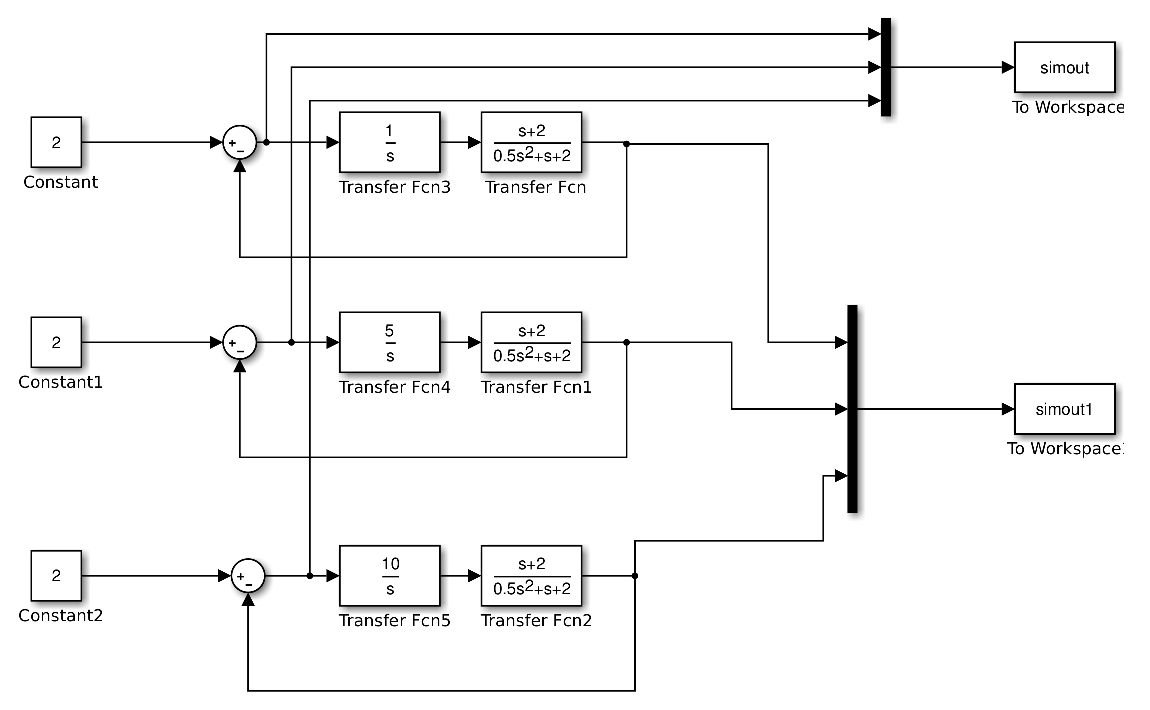
\includegraphics[width=\textwidth]{1/cxema_2.eps}
\caption{Структурная схема моделируемой  системы}
\end{figure}
Были получены переходные процессы для различных значений коэффициента  k.
На рисунке 8 приведены графики переходных процессов  для различных значений коэффициента  k.

\begin{figure}[H]
\centering
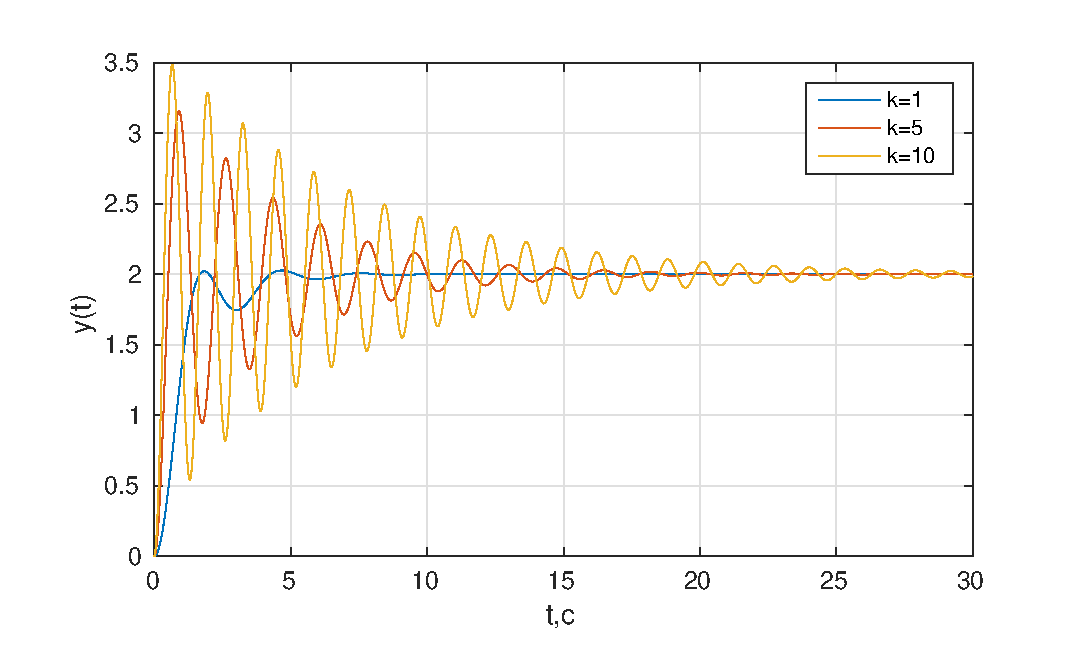
\includegraphics[width=\textwidth]{1/2_1y(t).eps}
\caption{Графики переходного процесса для k=1; k=5; k=10}
\end{figure}
Было получено предельное значение установившейся ошибки е.

\begin{figure}[H]
\centering
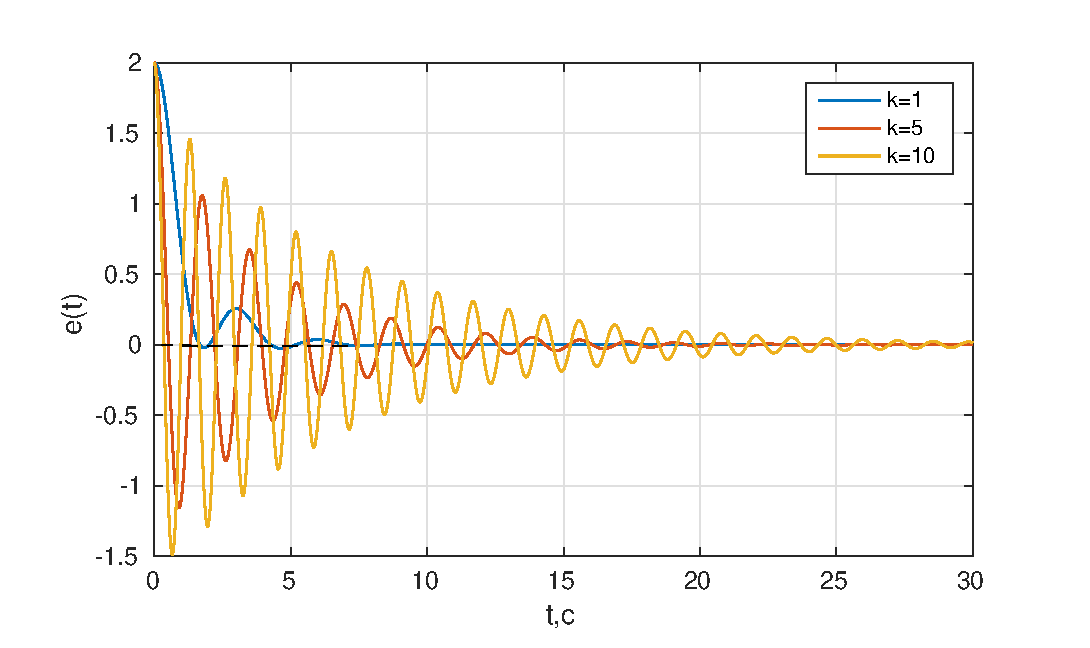
\includegraphics[width=\textwidth]{1/2_1e(t).eps}
\caption{Графики, изображающие предельное значение установившейся ошибки}
\end{figure}

Для системы с астатизмом 1 порядка значение установившейся ошибки е=0 (при g(t)=A).

\subsection{Исследование режима движения с постоянной скоростью: \\$g(t)=Vt$}

Были получены переходные процессы для различных значений коэффициента  k.
На рисунке 10 приведены графики переходных процессов  для различных значений коэффициента  k.
На рисунке 11 приведены графики установившейся ошибки.
\begin{figure}[H]
\centering
\includegraphics[width=\textwidth]{1/2_2y(t).eps}
\caption{Графики переходного процесса для k=1; k=5; k=10}
\end{figure}
Было получено предельное значение установившейся ошибки е.

\begin{figure}[H]
\centering
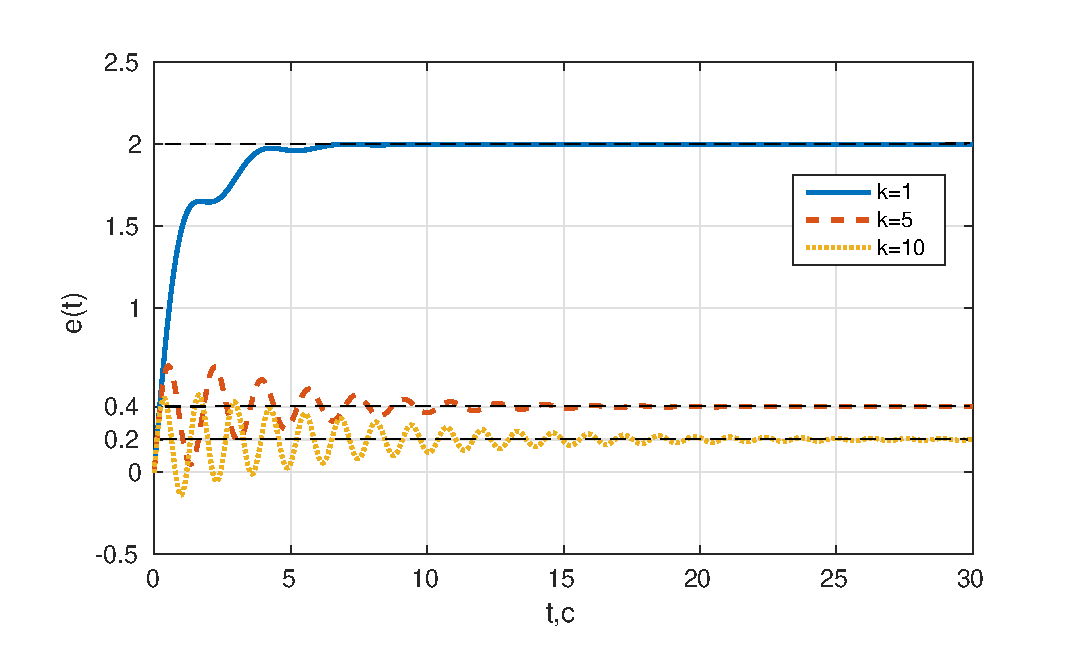
\includegraphics[width=\textwidth]{1/2_2e(t).eps}
\caption{Графики, изображающие предельное значение установившейся ошибки}
\end{figure}

Из рисунка видно, что
\\при k=1:  e=2
\\при k=5: е=0.4
\\при k=10: е=0.2.

С помощью расчета проверим получившееся на графике значения установившейся ошибки:
\begin{equation}
e=\frac{V}{k}
\end{equation}
Подставим полученные значения:
\\при k=1: e=2/1=2
\\при k=5: e=2/5=0.4
\\при k=10: e=2/10=0.2

Рассчитанные значения совпадают с получившимися значениями на графике.

\subsection{Исследование режима движения с постоянным ускорением: $g(t)=at^2/2$}

Были получены переходные процессы для различных значений коэффициента  k.
\\На рисунке 12 приведены графики переходных процессов  для различных значений коэффициента  k.

\begin{figure}[H]
\centering
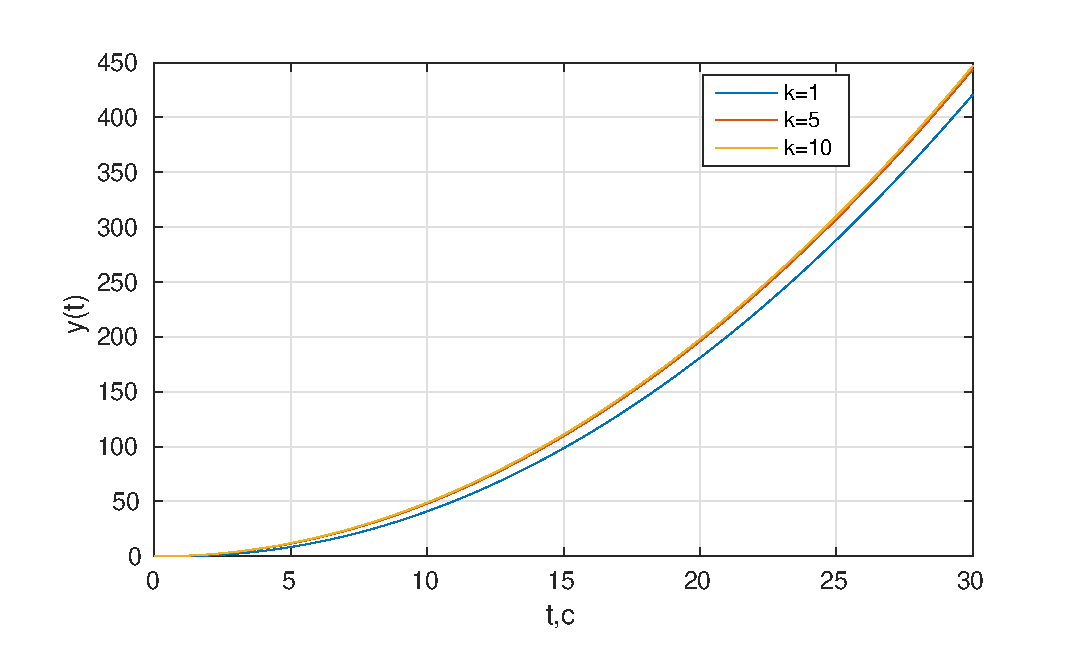
\includegraphics[width=\textwidth]{1/2_3y(t).eps}
\caption{Графики переходного процесса для k=1; k=5; k=10}
\end{figure}

\newpage
\begin{center}
\section{Исследование влияния внешних возмущений}
\end{center}
\par На рисунке 13 приведена структурная схема возмущенной системы.

\begin{figure}[H]
\centering
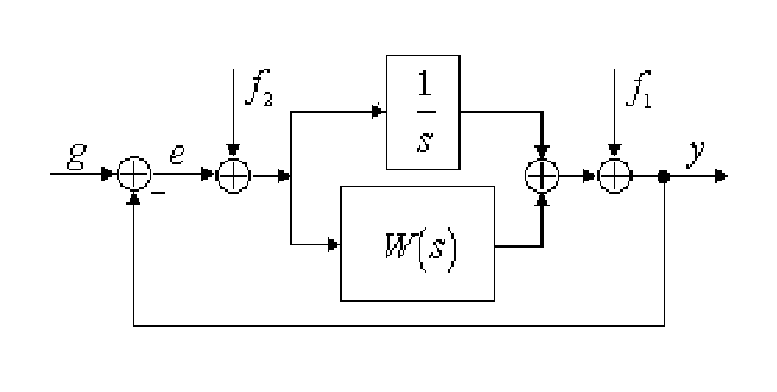
\includegraphics[width=0.5\textwidth]{1/444.eps}
\caption{Структурная схема возмущенной системы}
\end{figure}

На рисунке 14 приведена схема моделирования возмущенной системы.
На рисунке 15 представлен график переходного процесса. На рисунке 16 - график, изображающий предельное значение установившейся ошибки.
\begin{figure}[H]
\centering
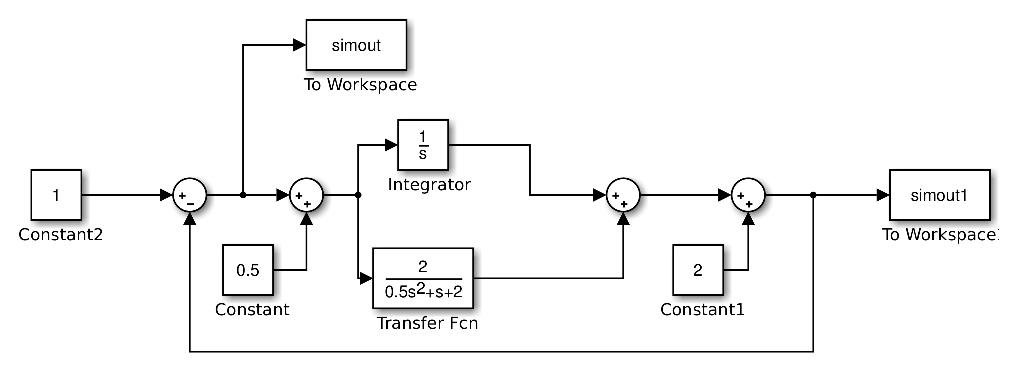
\includegraphics[width=\textwidth]{1/3.eps}
\caption{Схема моделирования возмущенной системы}
\end{figure}


Положим $f_{2}(t)=0$ и g(t)=1(t), получим переходный процесс:

\begin{figure}[H]
\centering
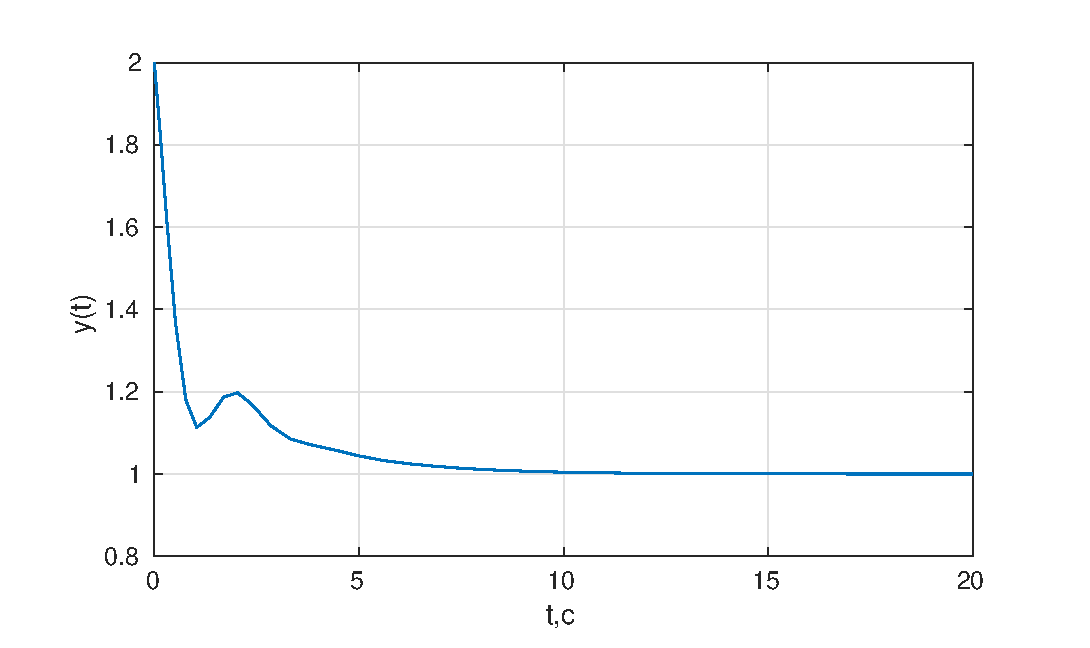
\includegraphics[width=\textwidth]{1/3_2y(t).eps}
\caption{График переходного процесса}
\end{figure}

Было получено предельное значение установившейся ошибки е.

\begin{figure}[H]
\centering
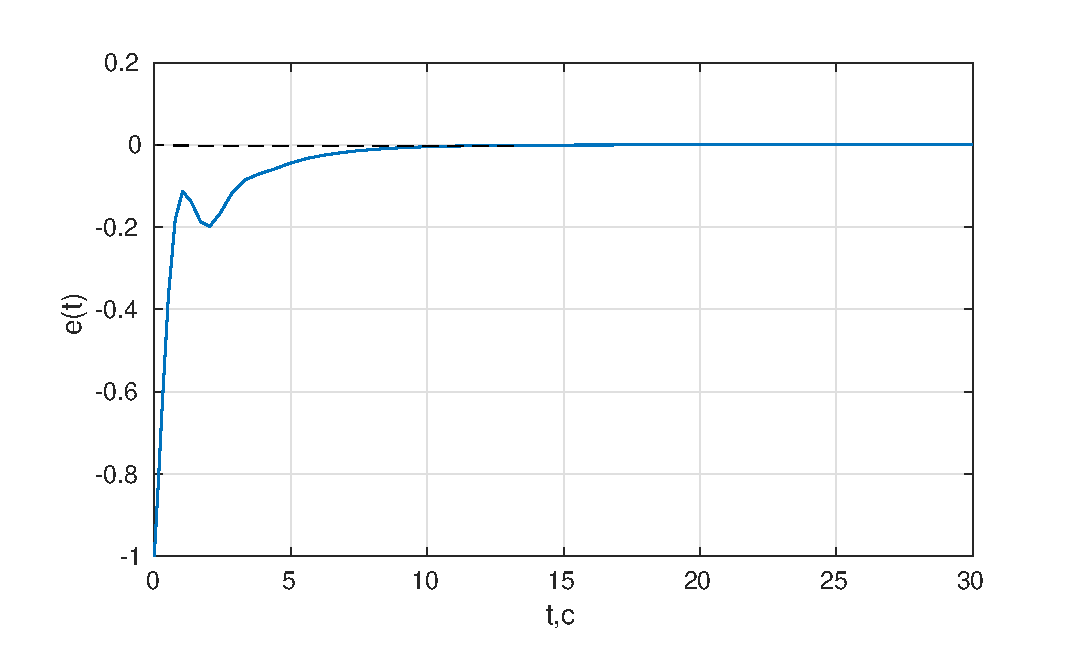
\includegraphics[width=\textwidth]{1/3_2e(t).eps}
\caption{График, изображающий предельное значение установившейся ошибки}
\end{figure}
Предельное значение установившейся ошибки е=0.

Положим $f_{1}(t)=0$ и g(t)=1(t), получим переходной процесс, который представлен на рисунке 17.
На рисунке 18 представлен график, изображающий предельное значение установившейся ошибки.

\begin{figure}[H]
\centering
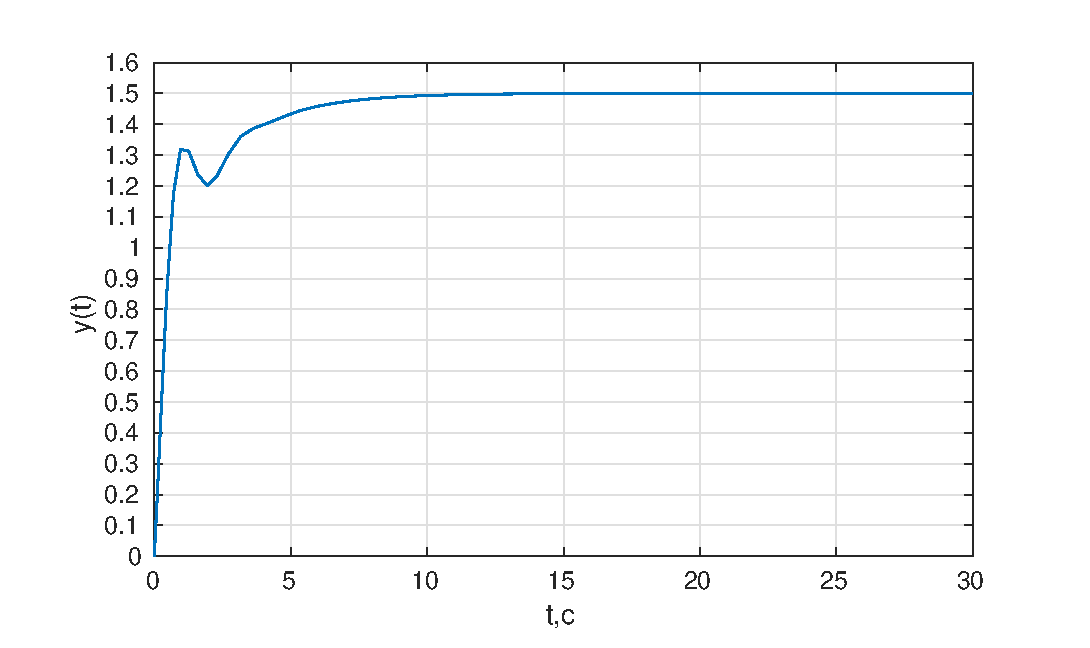
\includegraphics[width=\textwidth]{1/3_3y(t).eps}
\caption{График переходного процесса}
\end{figure}

Было получено предельное значение установившейся ошибки е.
\begin{figure}[H]
\centering
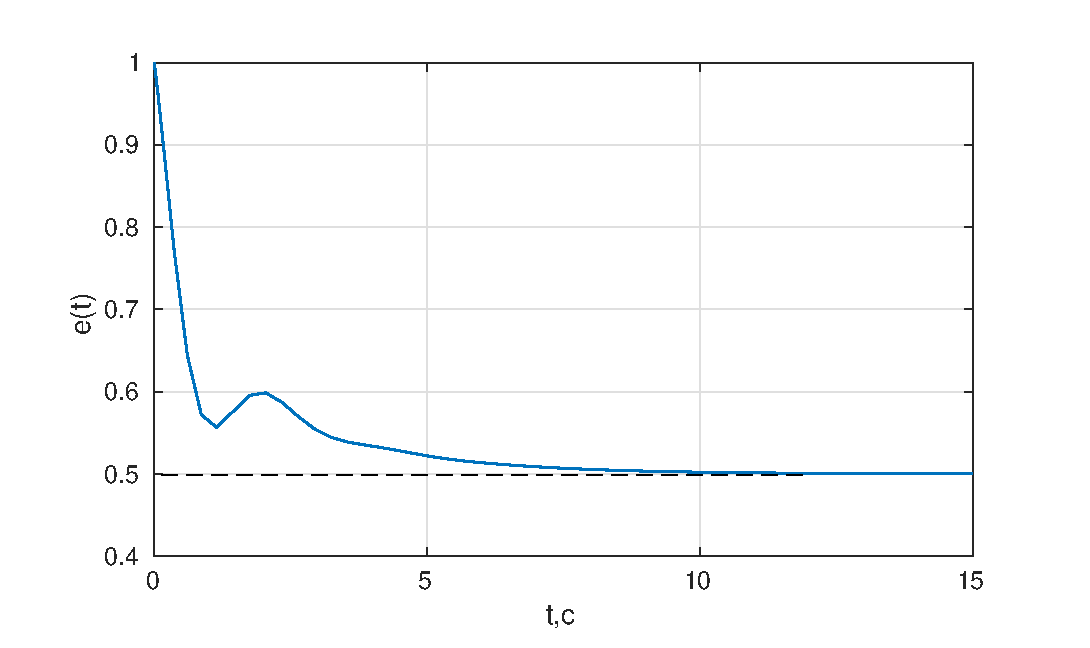
\includegraphics[width=\textwidth]{1/3_3e(t).eps}
\caption{График, изображающий предельное значение установившейся ошибки}
\end{figure}

Предельное значение установившейся ошибки е=0,5.
Проверим полученное значение:
\begin{equation}
e=F_{2}=f_{2}(t)
\end{equation}
\begin{center}
$e=F_{2}=f_{2}(t)=0,5$
\end{center}



Полученные значения установившейся ошибки сходятся, из этого можно сделать вывод, что полученное значение на графике — верно.

\newpage
\begin{center}
\section{Исследование установившейся ошибки при произвольном входном воздействии}
\end{center}

Была собрана структурная схема данной системы, которая представлена \\на рисунке 19.

\begin{figure}[H]
\centering
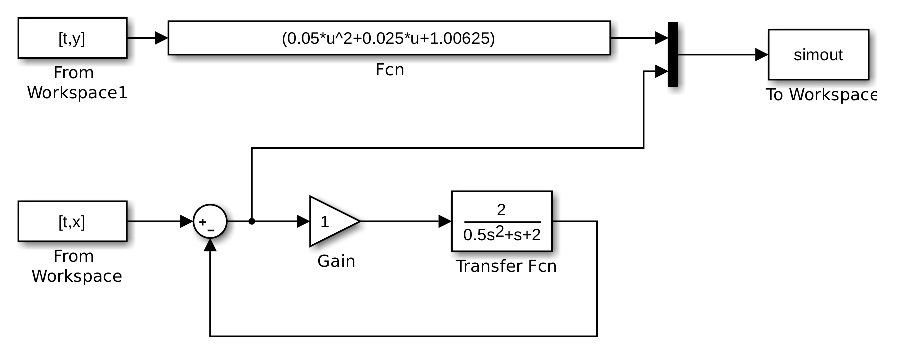
\includegraphics[width=\textwidth]{1/4.eps}
\caption{Структурная схема моделируемой  системы}
\end{figure}
Был получен переходный процесс в замкнутой системе, который представлен на рисунке 20.


\begin{figure}[H]
\centering
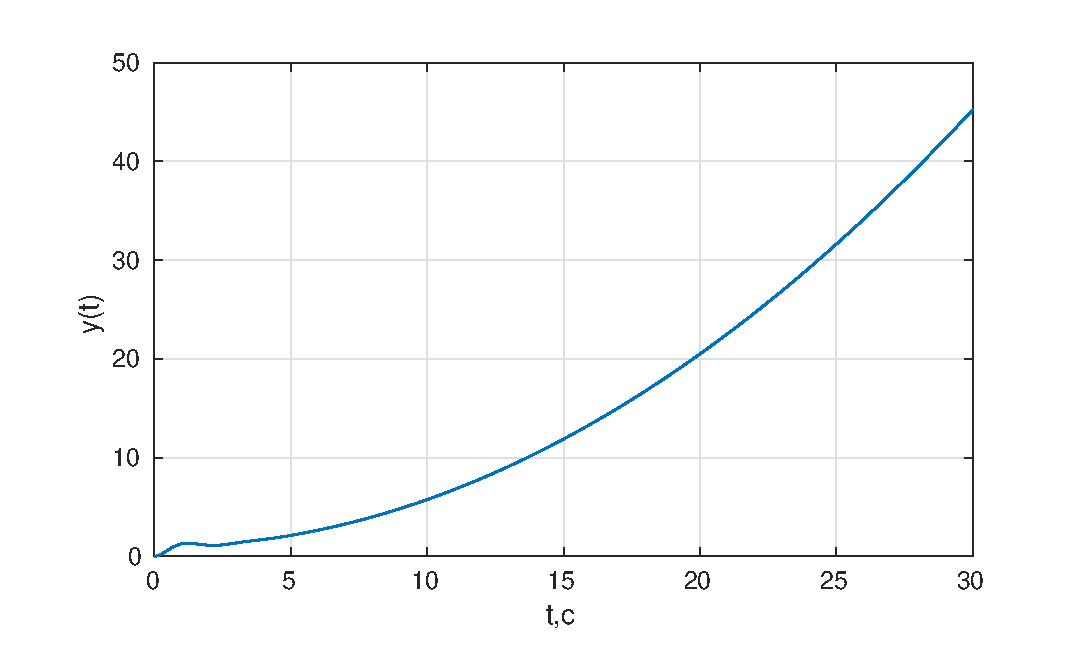
\includegraphics[width=\textwidth]{1/4_1y(t).eps}
\caption{Переходной процесс в замкнутой системе}
\end{figure}

На рисунке 21 представлен график, изображающий  установившуюся ошибку слежения.
\begin{figure}[H]
\centering
\includegraphics[width=\textwidth]{1/4_1e(t).eps}
\caption{График, изображающий  установившуюся ошибку слежения}
\end{figure}

Из графика видно, что установившаяся ошибка е=${\infty}$.

Получим приближенное аналитическое выражение для $e_{y}(t)$ , сохранив в ряде Тейлора три первых члена:
\begin{equation}
e(t)=c_{0}g(t)+c_{1}\dot{g}(t)+\frac{c_{2}}{2!}\ddot{g}(t)
\end{equation}
\begin{equation}
c_{i}=[\frac{d^i}{ds^i}\Phi_{e}(s)]
\end{equation}
		
\begin{align*}
    g(t) & = 2+0.1t^2 & \Phi_e(s)|_{s=0} & = \frac{0.5s^2+s+2}{0.5s^2+s+4}=0.5 \\
    \dot{g}(t) & = 0.2t & \left.\frac{d\Phi_e(s)}{ds}\right|_{s=0} & = \frac{8s+8}{(s^2+2s+8)^2}=0.125 \\
    \ddot{g}(t) & = 0.2 & \left.\frac{d^2\Phi_e(s)}{ds^2}\right|_{s=0} & = \frac{-24s^2-48s+32}{(s^2+2s+8)^3} = 0.0625 \\
\end{align*}\par

Подставим получившееся значения в выражение для ошибки:
\begin{equation}
e(t)=0.05t^2+0.025t+1.00625
\end{equation}
 Получили графики расчетной ошибки  и ошибки, вычисленной в ходе математического моделирования, которые представлены на рисунке 22.

\begin{figure}[H]
\centering
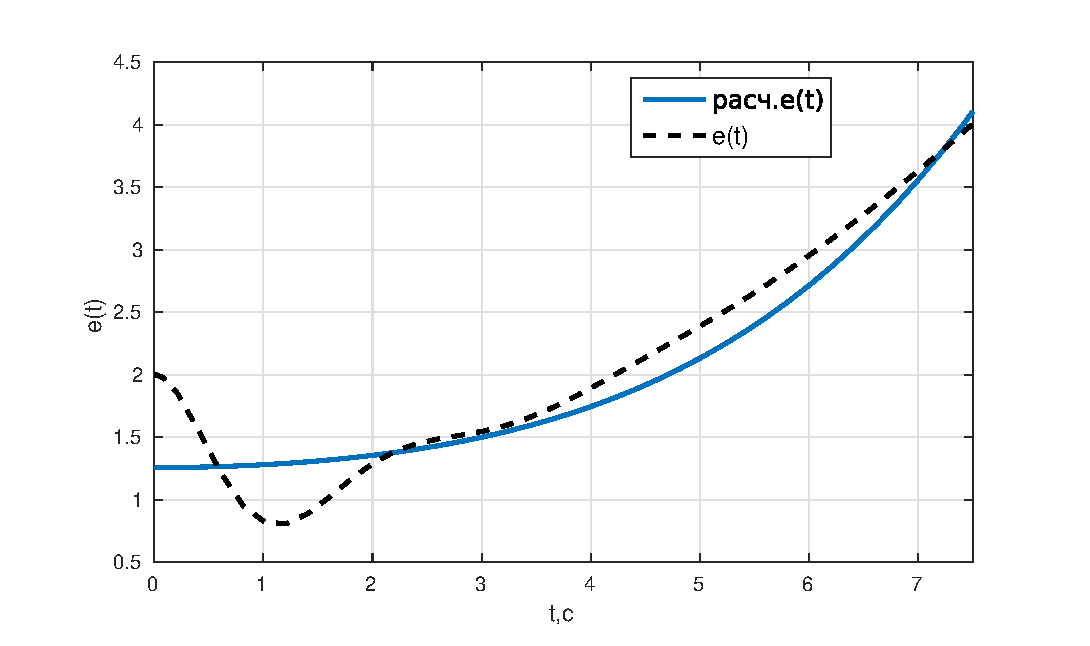
\includegraphics[width=\textwidth]{1/4_2e(t).eps}
\caption{Графики ошибок}
\end{figure}



\newpage

\section*{Вывод}

В данной лабораторной работе было проведено исследование системы с астатизмом нулевого и первого порядка; 
исследование влияния внешних возмущений; исследование установившейся ошибки при произвольном входном воздействии.
При исследовании системы с нулевым порядком астатизма в стационарном режиме работы значения установшейся ошибки были больше нуля.
А при исследовании системы с первым порядком астатизма в стационарном режиме работы значения установшейся ошибки стремились к нулю.
Полученные значения установившейся ошибки были проверены аналитически. 
При исследовании установившейся ошибки при произвольном входном воздействии - значение установившейся ошибки стремилось к бесконечности.


\end{document}
